\chapter{Implementation}
Für die Implementation dieser Bachelorarbeit wurden die im vorherigen Kapitel \ref{ch:konzepte_architektur} \nameref{ch:konzepte_architektur} beschrieben Konzepte angewendet.
\section{XML Daten Import}
Um mit den grossen Datenmengen in den vorhandenen XML Dateien effizient zu arbeiten, müssen diese Daten in eine Datenbank importiert werden. Dafür wurde ein Import Formular im Web Interface integriert, das im Hintergrund die Daten an einen Web Service sendet, der für den Import zuständig ist. Die Daten werden direkt beim Import aufbereitet, sodass die Abfrage der Daten schneller ist.
\section{Tiling der Daten}
\label{sec:tilingdataimplementation}
Während des Imports werden zwei verschiedene Vorberechnungen durchgeführt. Mit Hilfe dieser Aufbereitung ist es möglich, die Daten effizienter zu filtern. Dadurch wird die Antwortzeit einer Anfrage deutlich verkürzt.
\subsection{QuadKey}
Die erste Vorbereitung ist die Berechnung des QuadKeys. Wie in Kapitel \ref{ch:datentiles} \nameref{ch:datentiles} beschrieben, können mit Hilfe des QuadKey einzelne Bereiche der Welt eindeutig identifiziert werden. Wenn nun eine Anfrage an den Server gesendet wird, in der die Daten eines spezifischen QuadTiles angefordert werden, müssen die Links ebenfalls einen QuadKey besitzen, um danach zu filtern. Dafür werden die QuadKeys der beiden Nodes berechnet, die zu einem Link gehören. Der gemeinsame Präfix stellt nun den kleinstmöglichen QuadKey dar, in den der gesamte Link hineinpasst.\\
Wie in Abbildung \ref{pic:example_quadtile} bei Link 2 ersichtlich, kann eine Strasse in einem QuadTile ersichtlich sein, ohne dass sich beide Nodes in diesem Quadtile befinden. In diesem Beispiel hat Link 1 einen QuadKey von 010 und Link 2 von 01. Damit nun der Link 2 bei einer Abfrage der Daten des QuadTiles 010 auch mitgeliefert wird, müssen alle Strassen, die einen QuadKey besitzen, der einen Prefix des angeforderten QuadKeys darstellt, auch mitgeliefert werden. D.h. dass nun für die Abfrage des QuadTiles 010 alle Strassen, die den QuadKey 010, 01, 0 oder sogar einen leeren QuadKey (\glqq{}\grqq{}) besitzen mitgeliefert werden.
\begin{figure}[H]
\centering
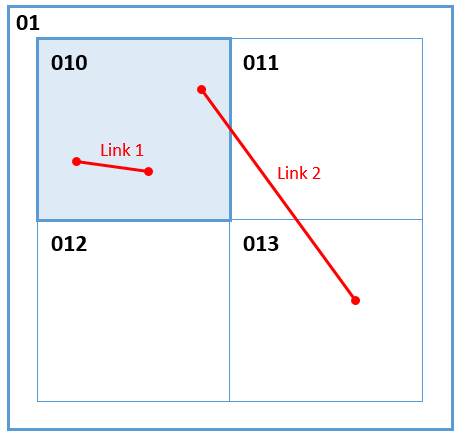
\includegraphics[height=9cm]{images/QuadTile_example.PNG}
\caption{Beispiel QuadTile}
QuadKey Link 1: 010\\QuadKey Link 2: 01
\label{pic:example_quadtile}
\end{figure}
\noindent
Der QuadKey ist eine sehr gute Technik um die Daten auf der Karte zu adressieren und dadurch eine Filterung der Daten durchzuführen. Zudem stellt diese Technik sicher, dass alle in einem gewissen QuadTile ersichtlichen Links sicher mitgeliefert werden.\\
Ein Nachteil dieser Technik ist es, dass bei höheren Zoomlevels Daten mitgeliefert werden, die bei einem vorherigen QuadTile bereits mitgeliefert wurden. Das User Interface verhindert zwar das neue Zeichnen von Duplikaten, jedoch werden dadurch Datensätze übertragen, die bereits gezeichnet sind und dadurch überflüssig sind. In den für diese Arbeit zur Verfügung stehenden Modellen hält sich die Menge von Links, die einen kleinen Präfix besitzen in Grenzen. Dadurch ebenfalls die Menge an Links, die mehrfach übertragen werden oder ausserhalb des sichtbaren Bereichs gezeichnet werden.
\newpage
\subsection{MinLevel}
Zusätzlich zu dem QuadKey wird beim Import für jeden Link der Mindest-Level (MinLevel) berechnet. Denn nur mit dem QuadKey würden alle Strassen in der aktuell angezeigten Bounding Box geladen werden, auch die eher kleineren Nebenstrassen. Aus diesem Grund wird beim Import ein MinLevel berechnet, der besagt, ab welchem Zoom Level in der Karte diese Strasse geladen wird. Dadurch ist es möglich, eine Strasse nach ihrer Wichtigkeit zu beurteilen und erst ab einem bestimmten Zoomlevel anzuzeigen.\\
Bei der Berechnung dieses Mindest-Levels wird in erster Linie auf die maximale  Geschwindigkeit geachtet. Die Geschwindigkeit sagt sehr viel über die Wichtigkeit der Strasse selbst aus. Eine Strasse mit einer hohen maximalen Geschwindigkeit, wie z.B. eine Autobahn, wird in diesem System als wichtig erachtet und dadurch bereits auf einem niedrigeren Zoomlevel angezeigt. Beim Level 10 und 14 wurden noch weitere Kriterien verwendet, um eine feinere Skalierung zu erhalten.\\
Der MinLevel einer Strasse wird wie folgt berechnet:\\[0.3cm]
\begin{tabular}{l c l} 
Level 10 & => & Geschwindigkeit > 30 m/s und Anzahl Spuren > 2 \\ 
Level 11 & => & Geschwindigkeit > 30 m/s  \\ 
Level 12 & => & Geschwindigkeit > 23 m/s \\ 
Level 13 & => & Geschwindigkeit > 14 m/s \\ 
Level 14 & => & Geschwindigkeit > 13 m/s und Kapazität >= 4000  \\ 
Level 15 & => & Geschwindigkeit > 13 m/s \\ 
Level 16 & => & Der Rest \\ 
\end{tabular}\\[0.4cm]
Alternativ zu den verwendeten Kriterien könnte die Berechnung des MinLevels auch mit Hilfe der Kapazität und zur feineren Abstufung der Anzahl Spuren der einzelnen Strassen durchgeführt werden. Dieses Verfahren hat jedoch eine unregelmässigere Verteilung auf die einzelnen Zoomlevels zur Folge. Aus diesem Grund wurde das Verfahren mit der Geschwindigkeit gewählt.
\newpage
\section{User Interface - Implementation}
Wie in Kapitel \ref{sec:uiconcept} \nameref{sec:uiconcept} beschrieben, muss das User Interface des Verkehrsmodell-Fallstudien-Editors einigen Anforderungen entsprechen. Dieses User Interface wird als Javascript Single Page Anwendung konzipiert und implementiert. Dies hat zum Vorteil, dass der Benutzer die Seite nie wechselt, sondern alle benötigten Elemente laufend nachgeladen werden. Dadurch erhält der Benutzer eine flüssigere User Experience. Die Web Applikation wird in eine Main View (Haupt-Anzeige) und mehrere Partial Views (Teil-Anzeigen) aufgeteilt. Die Partial Views werden im Play Framework als Route erfasst und mittels Javascript angefordert. Anschliessend werden diese Partial Views in einen Container geladen. Die Abbildung \ref{fig:mainviewpartialview} zeigt den Aufbau des User Interface mit einer eingezeichneten Partial View.
\begin{figure}[H]
\centering
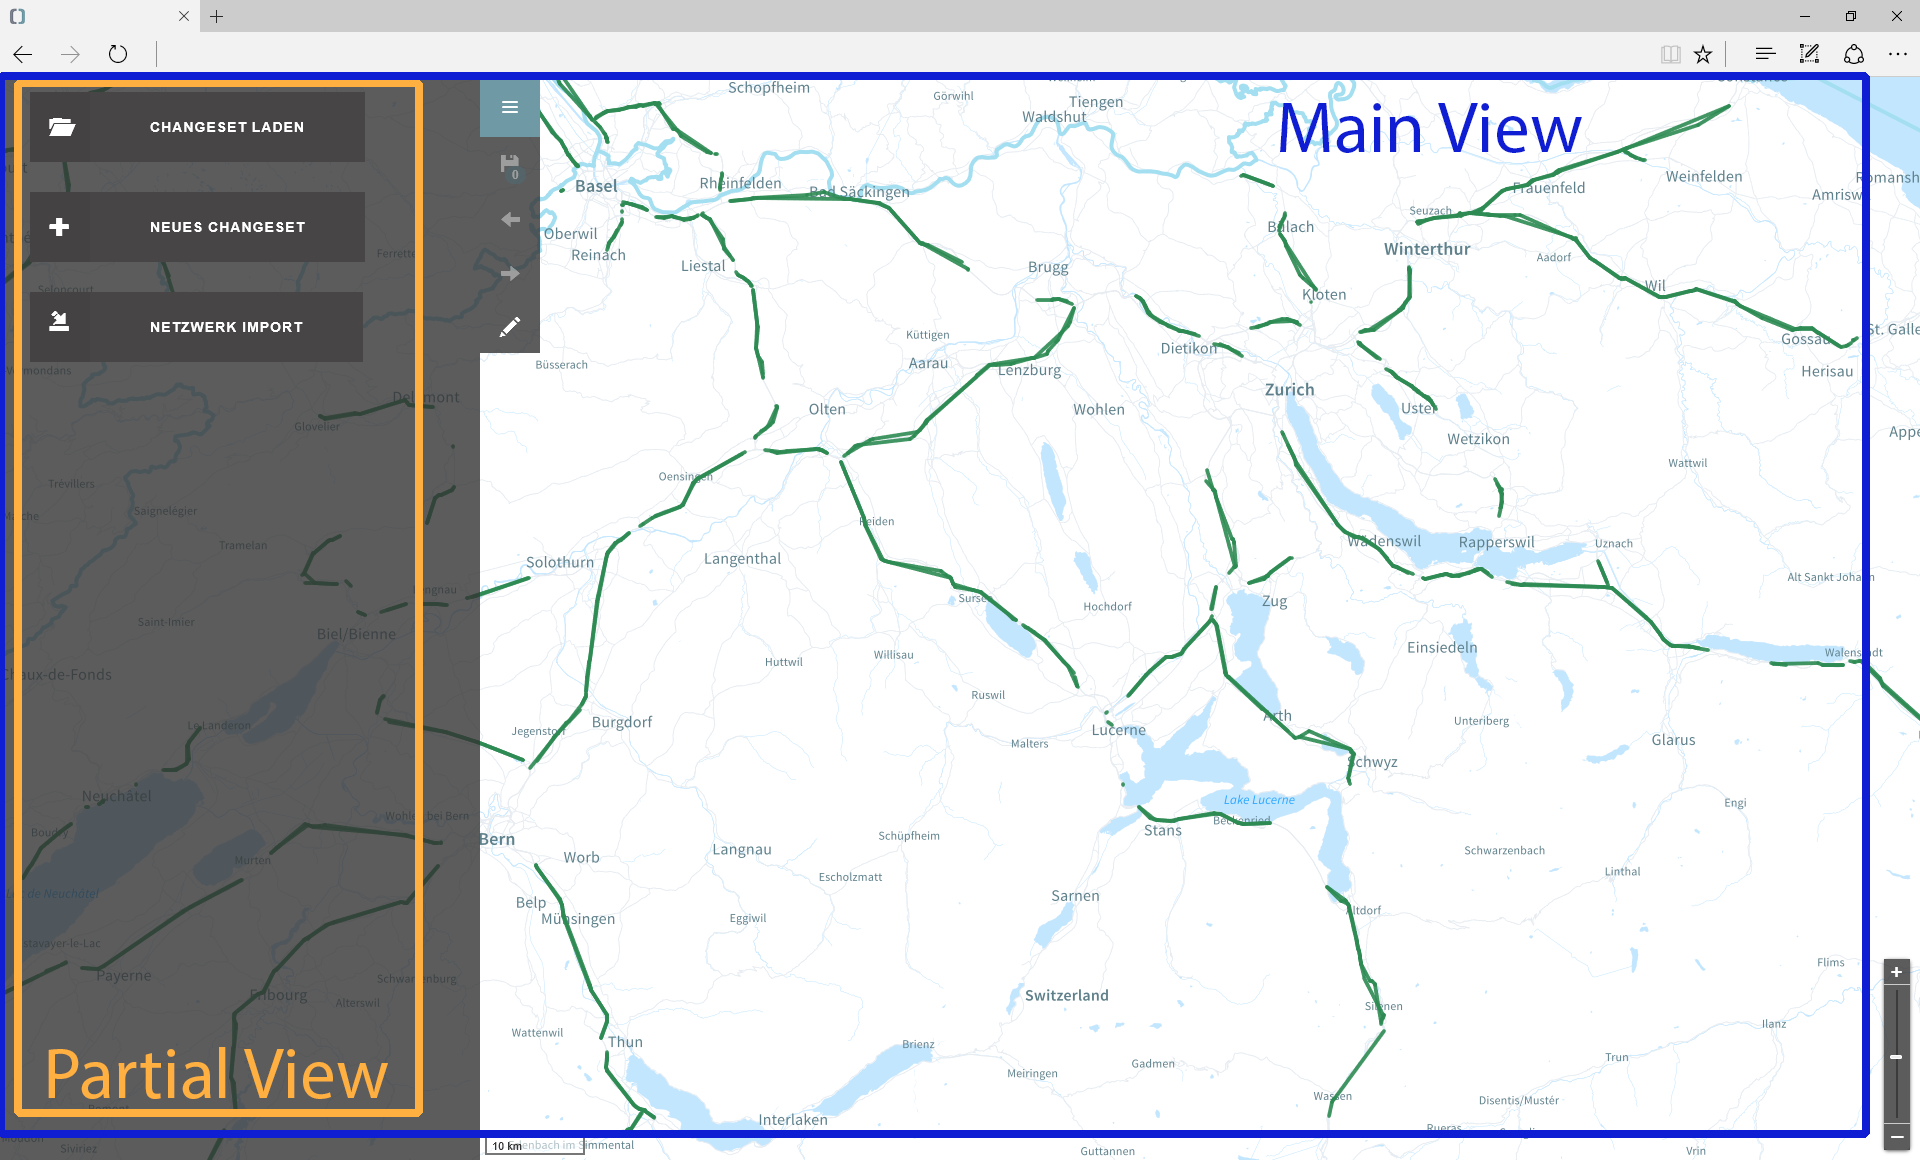
\includegraphics[height=6cm]{images/Mainviewpartialview.png}
\caption{User Interface mit eingezeichneter Partial View}
\label{fig:mainviewpartialview}
\end{figure}
\noindent
Wie in Abbildung \ref{fig:mainviewpartialview} ersichtlich, wurde der Karte viel Platz eingeräumt. Für die Darstellung der Karte wurde das Framework Leaflet \cite{Leaflet} sowie d3.js \cite{D3JS} verwendet. In der Kombination erlauben diese Frameworks die Erstellung einer Karte mit beliebigem Kartenmaterial im Hintergrund. Für die Karte wurde ein eigenes Kartendesign über Mapbox\cite{Mapbox} erstellt. Um zusätzlich zu der Karte eine Schicht mit den Daten aus dem Verkehrsmodell darzustellen, musste eine Erweiterung für Leaflet (TileLayer GeoJSON \cite{LeafletGeoJSON}) verwendet werden. Diese Erweiterung ermöglicht es, eine Schicht aufzubauen, welche die Daten für die Darstellung von einer URL nach dem OpenStreetMap Schema (x, y , zoom) anfordert und dabei GeoJSON als Antwortformat erwartet. Diese Library wurde gemäss den Anforderungen des Verkehrsmodell-Fallstudien-Editors erweitert. Mit Hilfe dieser Libray konnte das Konzept des Tiling der Daten (vgl. \ref{ch:datentiles} \nameref{ch:datentiles}) umgesetzt werden. Für die Interaktionen mit den einzelnen Editoren wird AngularJS \cite{AngularJS} Version 1.5 verwendet. AngularJS ermöglicht das Binding eines Models an Datenfelder und dadurch auch das Bearbeiten dieser Models. Z.B. wird beim Anklicken einer Strasse das Model der Strasse an das Edit-Menü gebunden und ermöglicht dadurch die Bearbeitung (vgl. Abbildung \ref{fig:editstreetattributes}).
\begin{figure}[H]
\centering
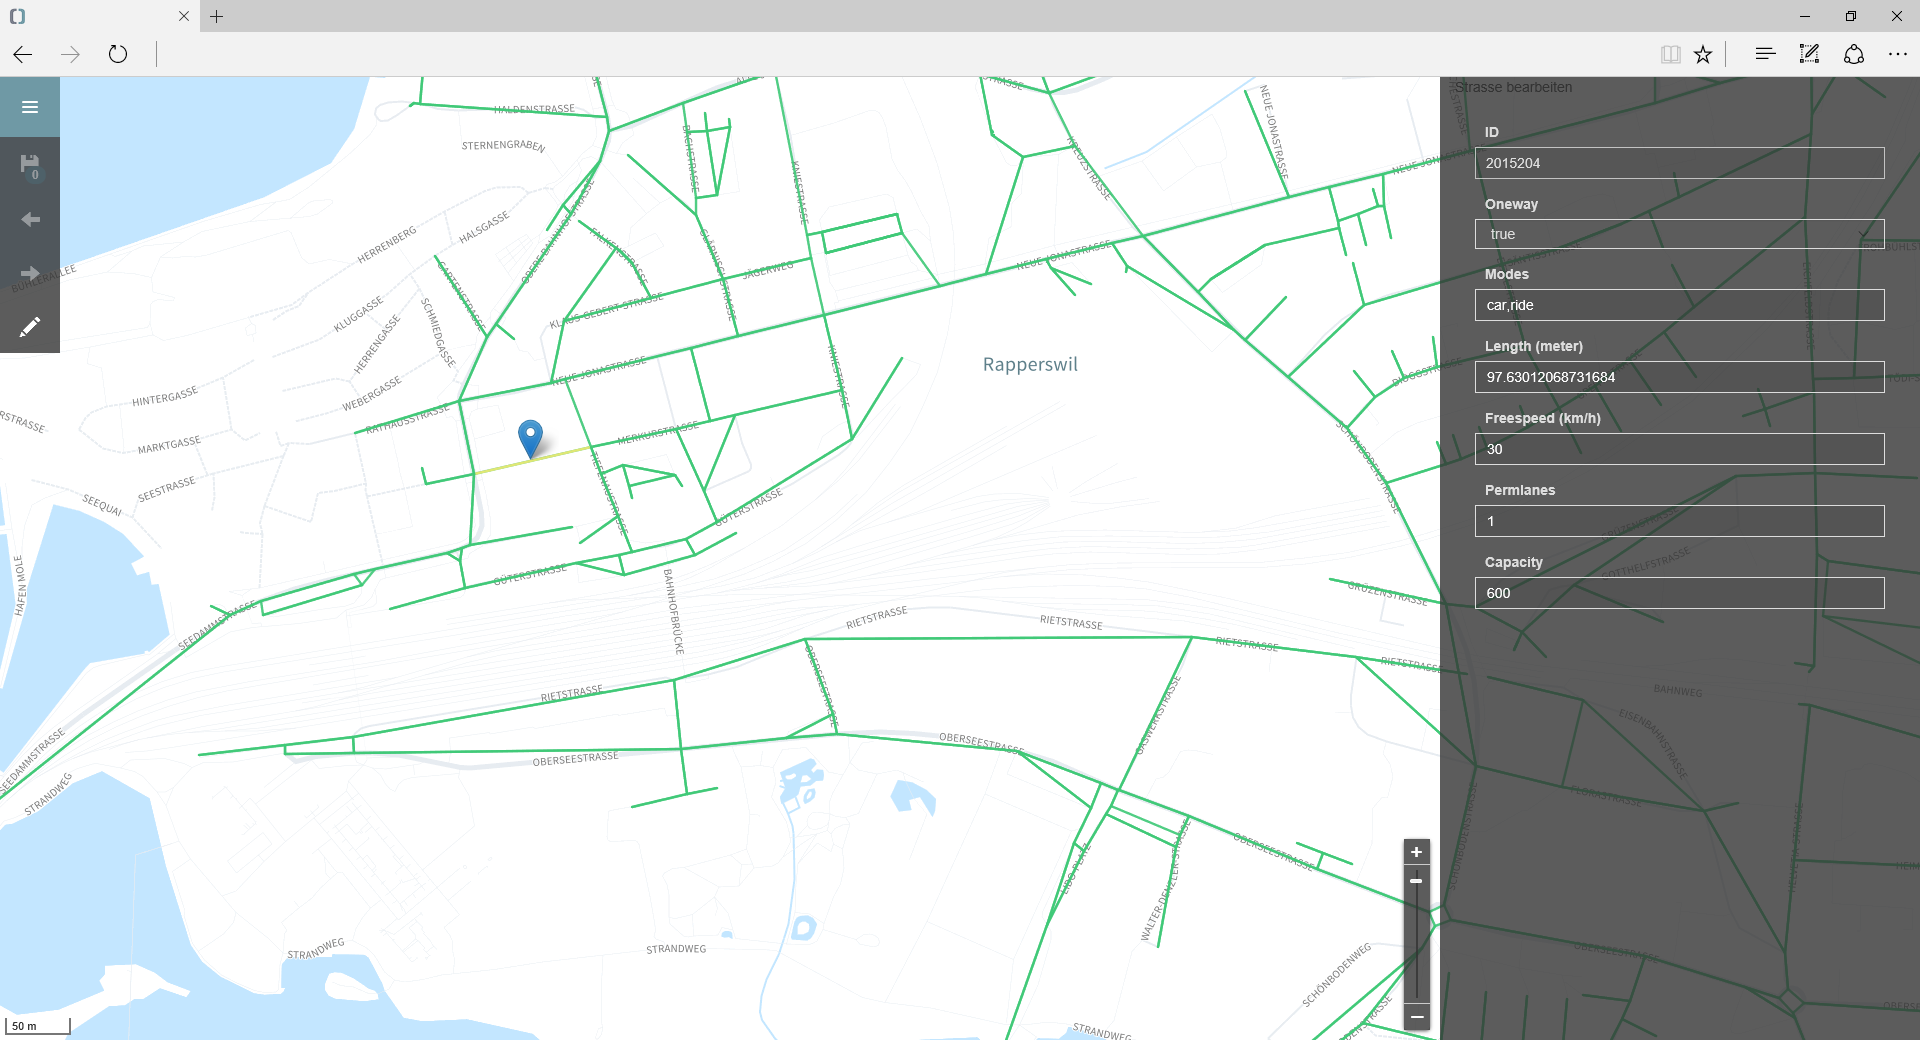
\includegraphics[height=6cm]{images/EditStreetattributes.png}
\caption{User Interface mit geöffnetem Editor für Strassenattribute}
\label{fig:editstreetattributes}
\end{figure}
\noindent
Um die Wegführung einer Strasse zu bearbeiten, kann eine Strasse angeklickt werden. Dabei öffnet sich ein Bearbeitungsfenster, in dem der Start und Endpunkt der Strasse mittels Klick auf den entsprechenden Node bearbeitet werden kann (vgl. Abbildung \ref{fig:editstreetdirection}). Nach der Bearbeitung wird die Strasse neu gezeichnet und hervorgehoben.\\
\begin{figure}[H]
\centering
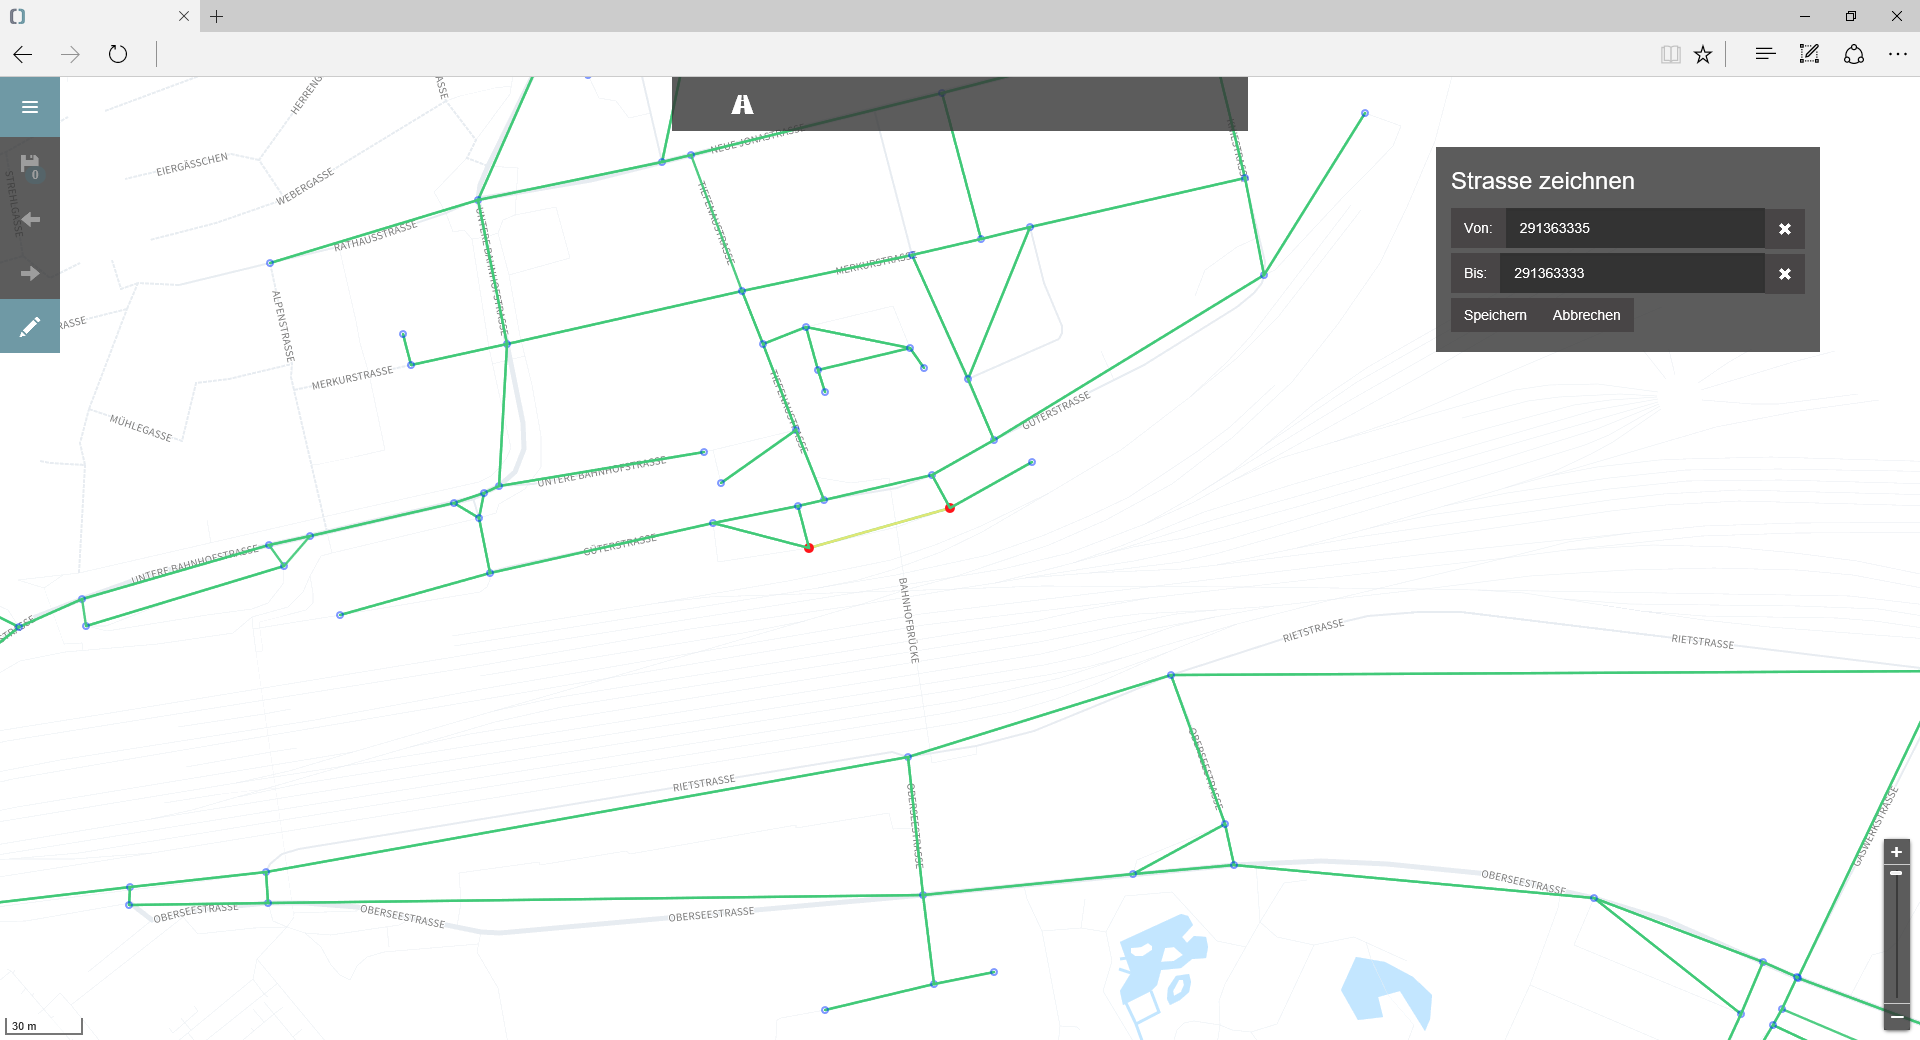
\includegraphics[height=6cm]{images/EditStreetdirection.png}
\caption{User Interface mit geöffnetem Editor für Strassenführung}
\label{fig:editstreetdirection}
\end{figure}
\noindent
Änderungen, welche über den Attribut-  oder Strassenführungseditor erstellt werden, werden auf einem Undo-Stack abgelegt. Dadurch können Änderungen über eine Undo-Funktion wieder rückgängig gemacht werden und über ein Redo wiederhergestellt werden. Das Changeset sowie der Undo- und Redo-Stack sind im Session Storage des Browser abgelegt. Dadurch gehen die Änderungen nicht verloren, solange die Browser Session noch offen ist. Wird der Browser geschlossen, gehen die Änderungen durch die Löschung der Session verloren. Der Benutzer kann seine Änderungen speichern, so dass sie in der Datenbank persistiert werden. Der Vorteil des Session Storage liegt darin, dass ein Benutzer die Seite neu laden kann oder ein Tab schliessen kann, ohne dass seine lokalen Änderungen verloren gehen.
\section{Performance Optimierungen}
\label{ch:performance}
Die Performance ist ein sehr wichtiger Faktor in dieser Arbeit. Ohne starke Performance kann die grosse Datenmenge in diesem Projekt nicht effizient dargestellt werden. Aufgrund dessen wurde einiges an Zeit in die Optimierung investiert. Zwei wichtige Faktoren haben grossen Einfluss auf die Performance dieser Web Applikation. Zum einen ist dies die Antwortzeit der einzelnen Abfragen der Daten. Diese Antwortzeit konnte durch mehrere Optimierungen, die in diesem Kapitel genauer beschrieben werden, deutlich verbessert werden. Dadurch konnten die nicht-funktionalen Anforderungen aus dem Kapitel \ref{ch:NFRs} \nameref{ch:NFRs} eingehalten werden.\\
Ein weiterer grosser Faktor ist das Rendering der Daten im Browser. In höheren Zoomlevels werden bis zu mehreren Tausend Links und Nodes im Browser dargestellt. Der Browser benötigt für das Rendering dennoch eine gewisse Zeit, auf die der Entwickler keinen grossen Einfluss hat. Es kann lediglich darauf geachtet werden, dass keine redundante Informationen vom Browser gerendert werden müssen.
\subsection{Caching}
Für die Anzeige der Strassen und Nodes werden sehr viele Daten übertragen. Damit die Daten bei mehrmaligem Anfragen nicht jedes Mal übertragen werden müssen, wird clientseitiges Caching eingesetzt.\\
Der Server gibt dem Client vor, wie er die Daten zwischenspeichern soll. Dafür wird bei jeder Antwort ein maximales Alter der Daten gesetzt. Wie in Abbildung \ref{pic:browser_cache} ersichtlich, speichert der Client die Daten in seinen lokalen Zwischenspeicher (Cache) und verwendet diese, solange das maximale Alter von einer Stunde noch nicht erreicht ist. Dies macht Sinn, weil sich die Stammdaten des Verkehrsmodells nur sehr selten ändern. Erst nach Ablauf dieser Stunde sendet der Browser erneut eine Anfrage an der Server.
\begin{figure}[H]
\centering
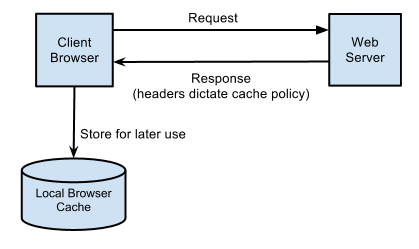
\includegraphics[height=6cm]{images/browser_cache.jpg}
\caption{Browser Zwischenspeicher Request (Cache) \cite{HTTPCacheHeaders}}
\label{pic:browser_cache}
\end{figure}
\newpage
\noindent
Nun liegt es am Server zu prüfen, ob die Daten, die sich im Cache des Clients befinden, noch aktuell sind. Dafür wird mit einem HTTP Entity Tag gearbeitet \cite{WikipediaETag}. Dieser setzt sich aus der x- und y-Koordinate, dem Zoom Level sowie aus dem Zeitstempel der letzten Bearbeitung der Daten zusammen. Durch diese unterschiedlichen Informationen ist der Entity Tag für jeden QuadTile eindeutig. Durch das zusätzliche Verwenden des Zeitstempels ist auch sichergestellt, dass sich der Entity Tag unterscheidet, sobald eine Änderung in den angeforderten Stammdaten auf dem Server vorliegt.\\
Jede Antwort, die zuvor an den Client gesendet wurde, wird mit diesem HTTP Entity Tag versehen. Beim erneuten Anfragen der Daten, wird dieser Entity Tag vom Client mitgesendet und mit dem berechneten, aktuellen Entity Tag der Daten auf dem Server verglichen. Wie in Abbildung \ref{pic:browser_etag} ersichtlich, wird vom Server der HTTP Status 304 (Not Modified) \cite{W3HttpStatus} gesendet, falls diese identisch sind. Dadurch weiss der Client, dass seine Daten noch aktuell sind. Wurden die Stammdaten auf dem Server geändert, stimmen die Entity Tags aufgrund des Zeitstempels der letzten Bearbeitung nicht mehr überein und der Server sendet die neuen Daten an den Client. Diese Daten werden dann vom Client wieder für eine Stunde zwischengespeichert und anschliessend beginnt der Prozess von vorne. Dieses Caching kann zu einer Inkonsistenz der Daten im Cache und dem Server führen. Jedoch wurde dieses Risiko bewusst eingegangen weil ein Update der Stammdaten nur sehr selten vorkommt. Zudem kann ein Update der Stammdaten zeitlich so gelegt werden, dass die Benutzer davon nicht betroffen sind.
\begin{figure}[H]
\centering
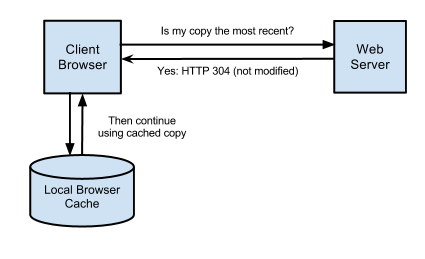
\includegraphics[height=6cm]{images/browser_etag.jpg}
\caption{HTTP Entity Tag Request \cite{HTTPCacheHeaders}}
\label{pic:browser_etag}
\end{figure}
\noindent
Durch dieses Verfahren ist sichergestellt, dass das Übertragen von Daten möglichst reduziert wird und dadurch Performance gewonnen wird. Das Beantworten eines Requests, der noch den selben Entity Tag verwendet und somit im Cache noch aktuell ist, benötigt ca. 50ms. Hingegen das erneute Senden würde ca. 200ms bis 300ms benötigen. Dadurch ist das Beantworten um de Faktor vier bis sechs schneller. Diese gewonnene Performance wird erst beim längeren Verwenden der Applikation ersichtlich, sobald bereits geladene Daten nicht mehr erneut geladen werden müssen.
\newpage
\subsection{Erneutes Zeichnen}
Die verwendete Library \glqq{}Leaflet GeoJSON Tile Layer\grqq{} \cite{LeafletGeoJSON}, die für das Abfragen der Daten in Tiles verantwortlich ist, wurde standardmässig so entwickelt, dass die Daten auf jedem Zoom Level neu gezeichnet werden. Im Rahmen dieser Arbeit wurde die Funktionalität erweitert, so dass die Strassen beim Hineinzoomen bestehen bleiben und lediglich die neuen Strassen dazu gezeichnet werden. Ebenfalls wurde die Library so angepasst, dass  beim Herauszoomen alle Strassen, die auf einem höheren Zoomlevel gezeichnet wurden, wieder entfernt werden. Dafür werden alle Schlüssel der gezeichneten Strassen mit dem dazugehörigen Zoomlevel, auf dem sie gezeichnet wurden, in eine Map< Zoomlevel, List<Schlüssel> > abgelegt. Dadurch kann die Library beim Herauszoomen alle Schlüssel, die zu einem Zoomlevel gehören, löschen.
\subsection{Datenbank Index}
Der Verkehrsmodell-Fallstudien-Editor arbeitet mit einer grossen Datenmenge, die in einer Datenbank gehalten wird. Die Abfrage einer Teilmenge der Daten benötigte bei einer Datenmenge von 4 Millionen Datensätzen bis zu drei Sekunden. Diese Antwortzeit ist deutlich zu lange und eine Auswertung des Ausführungsplans zeigte, dass die Indizes, die auf die einzelnen Zeilen gesetzt sind, nicht verwendet wurden.\\
Die Abfrage der Strassen beinhaltet eine LIKE Abfrage von SQL, die das Suchen von Strassen mit QuadKeys ermöglicht, die den QuadKey des aktuellen Tiles als Prefix besitzen. Speziell für SQL Abfragen mit einem LIKE Operator, bietet PostgreSQL eine Operator Klasse \glqq{}varchar\textunderscore pattern\textunderscore ops\grqq{}, die zusätzlich auf den Index des QuadKeys gesetzt werden kann. Dadurch wird der Index speziell für solche LIKE Abfragen vorbereitet und deutlich schneller. Nach dem Hinzufügen dieser Operator Klasse war der Zugriff auf die Daten zehn Mal so schnell und wir erreichten eine Zugriffszeit zwischen 100ms und 300ms.
\subsection{Datenbank Redundanz} \label{ch:redundance}
Die Daten in der Datenbank sind in eine Tabelle \glqq{}Links\grqq{} und eine Tabelle \glqq{}Nodes\grqq{} aufgeteilt. Bei der Abfrage werden sowohl die Parameter des Links als auch die Koordinaten der dazugehörigen Nodes benötigt. Dafür wurde zu Beginn ein klassischer SQL JOIN verwendet, um die beiden Tabellen miteinander zu verknüpfen. Durch die Analyse des Ausführungsplans wurde ersichtlich, dass dieser JOIN ca. die Hälfte der Ausführungszeit in Anspruch nahm. Um diese Zeit einzusparen, werden nun die Koordinaten der beiden Nodes direkt beim Import der Daten in die Tabelle der Links mit abgespeichert. Dadurch sind die Koordinaten der Nodes zwar redundant vorhanden, jedoch beschleunigt dies die Abfrage um den Faktor 2. Daher wurde die Redundanz der Daten in Kauf genommen.
\newpage
\section{Infrastruktur}
evtl. TODO
\subsection{Docker}
evtl. TODO
\subsection{Load Balancing}
evtl. TODO